\documentclass[xcolor=dvipsnames]{beamer} 
\setbeamertemplate{blocks}[rounded][shadow=false]

\usetheme{Madrid}

\setbeamertemplate{items}[square]
\setbeamertemplate{caption}[numbered]
\usecolortheme{beaver}
\usecolortheme{dolphin}
\usepackage{xkeyval}
\usepackage{todonotes}
\presetkeys{todonotes}{inline}{}
\usepackage{helvet}
\renewcommand{\familydefault}{\sfdefault}
\usepackage{float}
\usepackage[brazil]{babel}
\usepackage[utf8]{inputenc}
\usepackage{graphicx}
\usepackage{url}
\usepackage{float}     % para forçar a localizaçao das figuras (usando H no posicionamento, =Here)
\usepackage{subfigure}
\usepackage{mathtools} % setas com texto
\usepackage{multicol}
\usepackage{listingsutf8}
\usepackage{scalefnt}
\usepackage{ragged2e}
\usepackage{etoolbox, verbatim}
\usepackage[table,xcdraw]{xcolor}
\usepackage[dvipsnames,table,xcdraw]{colortbl}%colorir tabelas
\usepackage{pbox}%quebrar linha em uma célula da tabela
\usepackage{changepage}%mover a tabela pra esquerda

\setcounter{tocdepth}{2}
\setcounter{secnumdepth}{3}

\definecolor{mygray}{rgb}{0.4,0.4,0.4}
\definecolor{mygreen}{rgb}{0,0.8,0.6}
\definecolor{myorange}{rgb}{1.0,0.4,0}
\definecolor{pakistangreen}{rgb}{0.0, 0.4, 0.0}

\lstset{language=C++,
	basicstyle=\ttfamily\footnotesize, % Letra menor
	keywordstyle=\color{blue}\ttfamily,
	stringstyle=\color{red}\ttfamily,
	commentstyle=\color{green}\ttfamily,
	morecomment=[l][\color{pakistangreen}]{\#},
	showstringspaces=false,
	numbers=left,
	numbersep=5pt,
	numberstyle=\tiny\color{mygray},
	tabsize=2,
}

\renewcommand{\lstlistingname}{Código}

\let\olditem=\item% 
\renewcommand{\item}{\olditem \justifying}%

\beamertemplatenavigationsymbolsempty % tirar botões de controle

\title[Arquiteturas Paralelas e OpenMP]{Arquiteturas Paralelas e OpenMP}
\author[Ramos; Guimarães]{Natanael Ramos \\Rodolfo Labiapari Mansur Guimarães}
\institute[IFMG]{\begin{figure}
			\centering
			
\includegraphics[width=0.4\textwidth]{img/logo.jpg}
		\end{figure}}
%\institute[IFMG]{Instituto Federal de Educação, Ciência e Tecnologia de Minas Gerais - Campus Formiga}
\date[\today]{\today}

\begin{document}


\frame{\titlepage}

\AtBeginSubsection[] 
{
	\begin{frame}
	\frametitle{Sumário}
	\tableofcontents[
    currentsection, 
    currentsubsection, 
    hideothersubsections, 
    %sectionstyle=show/hiden, 
    subsectionstyle=show/shaded, ]
	\end{frame}
}






\section{Categorias de Arquiteturas de Computadores}
	\subsection{Introdução}
%\frame{
%    \Huge \color{blue} \bf  \centering Introdução
%}
\begin{frame}{Introdução}
	\begin{itemize}
	\item Taxonomia de Flynn descreve \textbf{categorias} de \textbf{arquiteturas de sistema de computadores}:
	\end{itemize}

	\begin{figure}[h]
		\centering
		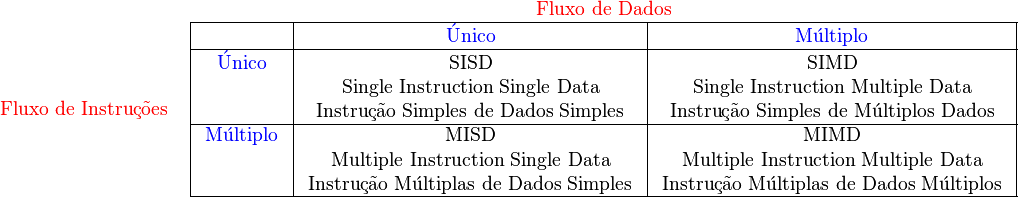
\includegraphics[width=1\textwidth]{img/tobias/taxonomia.png}
		\caption{Taxonomia de Flynn.}
		\label{fig:taxonomia}
	\end{figure}

\end{frame}

%\begin{frame}
%	\begin{itemize}
%		\item Nesta categorização encontra-se a diferenciação de
%		\begin{itemize}
%			\item Multicomputadores e Multiprocessadores; 
%			\item Memória Compartilhada e Memória Distribuída.
%		\end{itemize}
%		
%		\item Os tópicos abordados nesta apresentação serão:
%		\begin{itemize}
%			\item Single Instruction - Simple Data(SISD);
%			\item Single Instruction - Multiple Data(SIMD);
%			\item Multiple Instruction - Multiple Data(MIMD);
%			\item Memória Compartilhada;
%			\item Memória Distribuída;
%			\item ccNUMA;
%			\item Cluster;
%			\item Multiple Instruction - Simple Data(MISD);
%		\end{itemize}
%                
%                \bigskip
%                
%		\item Esta é \textit{válida} até os dias atuais.
%	\end{itemize}
%\end{frame}







%\frame{
%    \huge \color{blue}  \centering {\bf Single} Instruction - {\bf Single} Data (SISD) \\ e \\ {\bf Single} Instruction - {\bf Multiple} Data (SIMD)
%}
%\begin{frame}
%	\begin{itemize}
%		\item \textbf{SISD (Single Instruction - Single Data)}:
%		\begin{itemize}
%    		\item Executa apenas \textbf{1 instrução por ciclo de clock};
%    		\item Apenas 1 conjunto de dados ou operando;
%			\item Utiliza-se \textit{\bf pipeline} para melhorar eficiência;
%			\item Possui problemas com {\it branchs}.
%		\end{itemize}
%		\item \textbf{SIMD (Single Instruction - Multiple Data)}:
%		\begin{itemize}
%			\item Com a \textbf{computação numérica}, permitiu-se o uso de vários conjuntos de dados \textbf{com o mesmo operador}.
%			\item A arquitetura que executa uma instrução para vários dados é chamada de \textbf{vetorial} (Computadores 
%			Vetoriais) e de forma {\it parecida} \textbf{pipeline escalar}.
%			\item Entretanto, eles trabalham com \textbf{vetores de dados} processados em \textbf{1 ciclo}:
%			\begin{itemize}
%				\item Um computador vetorial com \textit{64 elemento} de vetores pode gerar até {\it 64 resultados por ciclo};
%				\item Diferentemente do processador escalar que necessitaria de exatos de 64 ciclos prévios;
%			\end{itemize}
%	
%				\bigskip
%
%		\end{itemize}
%		%\item Categorizações SISD e SIMD {\it não} fazem parte do conceito de multiprocessadores/multicores {\it nem} necessitam de compartilhamento de memória.
%	\end{itemize}
%\end{frame}
%\frame{
%    \Huge \color{blue} \bf  \centering Single Instruction - Single Data (SISD)
%}
%\begin{frame}{Single Instruction - Single Data (SISD)}
%	\begin{itemize}
%		\item Arquitetura que possui tipo de execução mais simples:
%		\begin{itemize}
%    		\item Executa apenas 1 instrução por ciclo de clock.
%    		\item Apenas 1 conjunto de dados ou operando.
%		\end{itemize}
%
%		\item Também chamado de \textbf{Computação Escalar}. 
%	\end{itemize}
%
%	\begin{figure}[h]
%		\centering
%		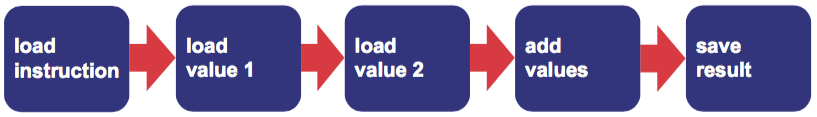
\includegraphics[width=0.9\textwidth]{img/tobias/sisd1.png}
%		\caption{Soma de 2 operando.}
%		\label{fig:sisd1}
%	\end{figure}
%
%	\begin{itemize}
%		\item \textbf{Problema:} Para adicionar 5 pares de números, necessita de $n * 5$ clocks.
%		%\item Cada um das etapas mostradas na Figura~\ref{fig:sisd1} possui sub-etapas piorando a execução da máquina.
%	\end{itemize}
%
%\end{frame}
%
%
%\begin{frame}{Single Instruction - Single Data (SISD)}
%    \begin{itemize}
%		\item Então, pra tornar mais eficiente, utiliza-se \textbf{pipelining}.
%%		\item Por exemplo,
%%		\begin{itemize}
%%			\item  Se existe \textbf{unidade funcional} para os 5 passos da soma, então gasta-se 5 ciclos.
%%			\begin{itemize}
%%    		    \item Se todas as unidades estiverem ocupadas, existirá um resultado a cada ciclo. 
%%			\end{itemize}
%%
%%    		\item Para a soma de $N$ números teríamos somente $(n - 1) + 5$ ciclos de clock.
%%		\end{itemize}
%%
%%	\end{itemize}
%%
%%\end{frame}
%%
%%
%%\begin{frame}{Single Instruction - Single Data (SISD)}
%%    \begin{itemize}
%		\item Instruções normalmente possuem mais de 5 passos implicando em pipelines longos nos processadores reais:
%		\begin{itemize}
%			\item Implicam também em frequência de clock alta.
%		\end{itemize}
%
%		\item Entretanto, longos pipeline possuem problemas com desvios:
%		\begin{itemize}
%			%\item Deve ser \textbf{esvaziado} e \textbf{preenchido} novamente;
%			%\item Há um número de ciclos (igual ao tamanho do pipeline) para que possa ficar eficiente novamente.
%
%			\item Deseja-se que o \textbf{número de desvios} seja \textbf{pequeno}; ou 
%			\item \textbf{Reposicionamento} dos desvios de forma inteligente:
%			\begin{itemize}
%			    \item \textit{Branch prediction}.
%			\end{itemize}
%
%		\end{itemize}
%
%%	\end{itemize}
%%
%%\end{frame}
%%
%%
%%\begin{frame}{Single Instruction - Single Data (SISD)}
%%    \begin{itemize}
%		\item Processadores podem ter um \textbf{desempenho superior} utilizando combinações de \textbf{vários pipelines} (Processadores Superescalares):
%		\begin{itemize}
%			\item \textbf{Cálculos Lógico/Aritiméticos} (ALU) são separados de \textbf{Pontos Flutuantes} (FPU).
%			\item Normalmente, FPU é dividido em uma unidade para adição e outra para multiplicação.
%			\begin{itemize}
%			    \item Além de unidades de divisão e computação de raiz quadrada.
%			\end{itemize}
%
%		\end{itemize}
%
%		%\item Hoje, o ganho deste tipo de arquitetura está nos \textbf{vários pipelines} no qual podem ser usados \textbf{ao mesmo tempo}.
%	\end{itemize}
%
%\end{frame}
%
%
%
%
%
%
%
%
%\frame{
%    \Huge \color{blue} \bf  \centering Single Instruction - Multiple Data (SIMD)
%}
%
%\begin{frame}{Single Instruction - Multiple Data (SIMD)}
%	\begin{itemize}
%		\item Com a \textbf{computação numérica}, permitiu-se o uso de vários conjuntos de dados \textbf{com o mesmo operador}.
%		\item A arquitetura que executa uma instrução para vários dados é chamada de \textbf{vetorial} (Computadores Vetoriais) e de forma parecida \textbf{pipeline escalar}.
%		\item Entretanto, eles trabalham com \textbf{vetores de dados} processados em \textbf{1 ciclo}:
%		\begin{itemize}
%			\item Um computador vetorial com 64 elemento de vetores pode gerar até 64 resultados por ciclo;
%			\item Diferentemente do processador escalar que precisa de 64 ciclos prévios;
%		\end{itemize}
%
%	\end{itemize}
%
%	
%\end{frame}
%
%
%\begin{frame}{Single Instruction - Multiple Data (SIMD)}
%	\begin{itemize}
%		\item Pra utilizar todo seu desempenho de processamento, os cálculos por ele executado \textbf{também devem ser 
%		naturalmente vetoriais} e utilizar \textbf{todos os recursos disponíveis}.
%%		\item Usados no âmbito de computação com alta performance:
%%		\begin{itemize}
%%			\item Permite alta performance com baixa frequência de clock.
%%		\end{itemize}
%
%%	\end{itemize}
%%
%%\end{frame}
%%
%%
%%\begin{frame}{Single Instruction - Multiple Data (SIMD)}
%%	\begin{itemize}
%%		\item Estão desaparecendo lentamente com o passar dos anos:
%%		\begin{itemize}
%			\item São \textbf{complexos} e \textbf{caros} e não suportam bem \textbf{problemas não-vetoriais}.
%		    \item Computadores escalares são baratos e possuem alta frequência de clock.
%%		\end{itemize}
%
%%		\item Computadores vetoriais não foram disseminados totalmente:
%%		\begin{itemize}
%%			\item Com o Pentium III, a Intel introduziu o SSE (Streaming SIMD Extension) que possuía um conjunto de instruções vetoriais;
%%			\item Logo em seguida:
%%			\begin{itemize}
%%			    \item SSE2 com o Pentium IV;
%%			    \item SSE3 com o Pentium IV Pescott.
%%			\end{itemize}
%%
%%		\end{itemize}
%
%	\end{itemize}
%
%\end{frame}






	\subsection{Memória Compartilhada, Distribuída e suas Combinações}
%\frame{
%    \Huge \color{blue}  \centering {\bf Multiple} Instruction - \\ {\bf Multiple} Data (MIMD)
%}
\begin{frame}{Multiple Instruction - Multiple Data (MIMD)}
	\begin{itemize}
		%\item Até então foi considerado operações que executam em \textbf{1 ciclo de clock}.
		%\item Isso aplica-se a todos os computadores que possui \textbf{1 processador de 1 core}.
		\item Arquiteturas com vários cores ou vários processadores \textbf{independente da classe (escalar/vetor)}, são declaradas MIMD.
		\item Todos os processadores de alta performance pertence a essa categoria.

				\bigskip

		\item Pode ser subdividida de acordo com a arquitetura de memória:
		\begin{enumerate}
			\item Memória Compartilhada;
			\item Memória Distribuída;
			\item Combinações.
		\end{enumerate}

	\end{itemize}

\end{frame}








\begin{frame}{Memória Compartilhada - SM-MIMD}
	\begin{itemize}
		\item MIMD com memória compartilhada (SM-MIMD) são processadores que são conectados \textbf{num barramento comum de memória RAM}.
		\item Também pode ser nomeado como Multiprocessamento Simétrico
		\begin{itemize}
			\item \textbf{Processadores devem ser idênticos} e possuem \textbf{igual acesso à memória};
			%\item Podem ser encontrados em PC e pequenos servidores.
		\end{itemize}

	\end{itemize}

\end{frame}


\begin{frame}{Memória Compartilhada - SM-MIMD}
    \begin{figure}[h]
    	\centering
    	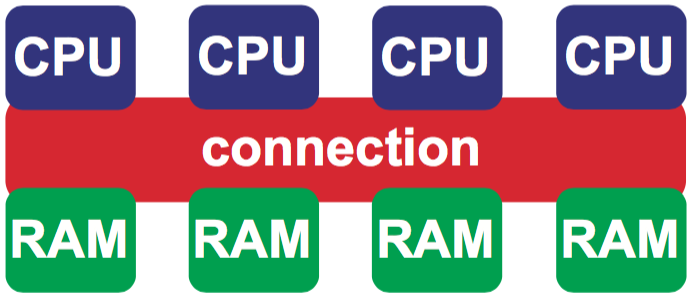
\includegraphics[width=0.95\textwidth]{img/tobias/sm-mimd.png}
    	\caption{\textbf{Modelo} MIMD com compartilhamento de memória.}
    	\label{fig:sm-mimd}
    \end{figure}

\end{frame}


\begin{frame}{Memória Compartilhada - SM-MIMD}
    \begin{figure}[h]
    	\centering
    	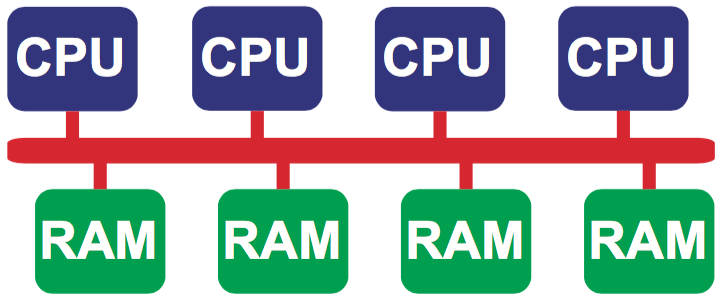
\includegraphics[width=1\textwidth]{img/tobias/sm-mimd2.png}
    	\caption{MIMD com compartilhamento de memória por meio de {\bf 1 único barramento}.}
    	\label{fig:sm-mimd2}
    \end{figure}

\end{frame}


\begin{frame}{Memória Compartilhada - SM-MIMD}
	\begin{itemize}
		\item \textbf{Vantagem:}
		\begin{itemize}
	    	\item Expansibilidade.
		\end{itemize}

			\bigskip

		\item \textbf{Desvantagem:}
		\begin{itemize}
		    \item Todos devem compartilhar a mesma largura de banda, mesmo acessando diferentes módulos de memória.
		\end{itemize}

		\item Com isso, a conexão entre processador e memória torna-se item essencial na eficiência.
	\end{itemize}

\end{frame}


\begin{frame}{Memória Compartilhada - SM-MIMD}
    \begin{figure}[h]
    	\centering
    	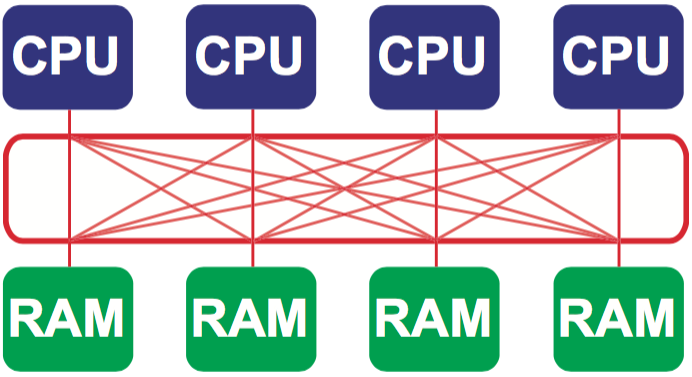
\includegraphics[width=1\textwidth]{img/tobias/sm-mimd3.png}
    	\caption{MIMD com compartilhamento de memória por meio de um {\bf comutador}.}
    	\label{fig:sm-mimd3}
    \end{figure}

\end{frame}


\begin{frame}{Memória Compartilhada - SM-MIMD}
	\begin{itemize}

		\item Computadores de alta performance e \textit{workstations}.

						\bigskip
		\item \textbf{Vantagem:}
		\begin{itemize}
		    \item Todos os processadores podem comunicar com as memórias tornando o \textit{software} fácil para desenvolvimento e eficiente para o uso.
		\end{itemize}

			\bigskip

		\item \textbf{Desvantagem:}
		\begin{itemize}
			\item Possuem um alto \textbf{grau de complexabilidade} quando muitas conexões devem ser feitas.
			\begin{itemize}
			    \item Grafo Bipartido Completo: Para $m + n$ vértices, existe $m*n$ arestas.
			    \item Utiliza-se uma variante dessa com comutadores multi-estágios para reduzir este problema.
			\end{itemize}
		\end{itemize}

	\end{itemize}

\end{frame}








\begin{frame}{Memória Distribuída - DM-MIMD}
	\begin{itemize}
		%\item Ao utilizar memória compartilhada, torna-se complicado a tarefa de acrescentar arbitrariamente o número de memória e processadores.
		%\item E sobre este problema, existe outro meio no qual utiliza-se \textbf{Memória Distribuída} (DM-MIMD).
		%\begin{itemize}
			\item Cada processador \textbf{possui sua memória local} e são \textbf{conectados entre si}.
			\item As exigências nesta rede são mais baixa
			\begin{itemize}
			    \item Entretanto a troca de informação é \textbf{mais lenta}.
			\end{itemize}
		%\end{itemize}

	\end{itemize}

\end{frame}


\begin{frame}{Memória Distribuída - DM-MIMD}
    \begin{figure}[h]
    	\centering
    	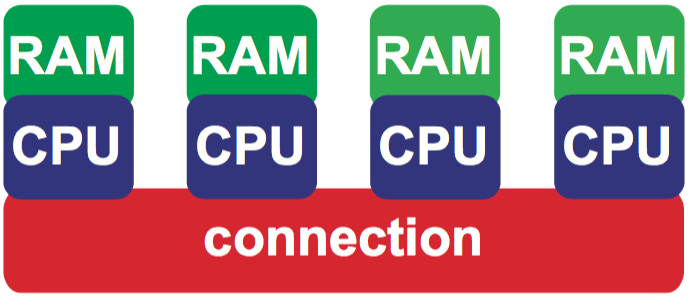
\includegraphics[width=1\textwidth]{img/tobias/dm-mimd.png}
    	\caption{MIMD com distribuição de memória.}
    	\label{fig:dm-mimd}
    \end{figure}

\end{frame}


%\begin{frame}
%    \begin{figure}[h]
%    	\centering
%    	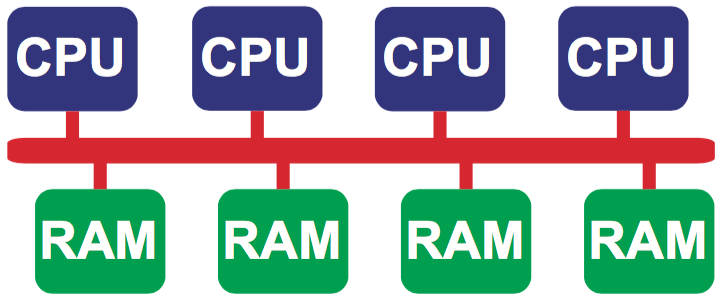
\includegraphics[width=0.6\textwidth]{img/tobias/sm-mimd2.png}
%    	\caption{Compartilhamento de memória por meio de {\bf 1 único barramento}.}
%    	\label{fig:sm-mimd2}
%    \end{figure}
%
%    		\bigskip
%
%    \begin{figure}[h]
%    	\centering
%    	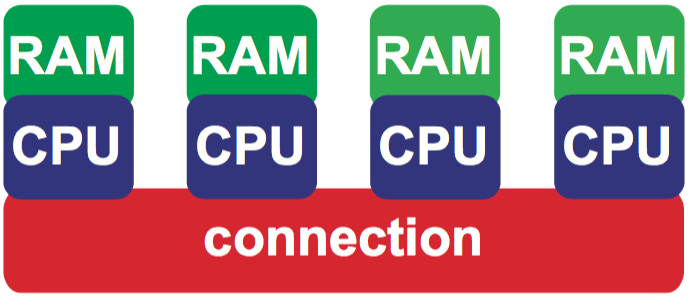
\includegraphics[width=0.6\textwidth]{img/tobias/dm-mimd.png}
%    	\caption{Distribuição de memória.}
%    	\label{fig:dm-mimd}
%    \end{figure}
%
%\end{frame}

\begin{frame}{Memória Distribuída - DM-MIMD}
	\begin{itemize}
		%\item Necessita de mais esforço na \textbf{programação} do que no \textbf{sistema de memória compartilhada}.
		\item Podem ser expandidas facilmente e utilizar modelos de processador/memória diferentes.
		\item O uso de milhares de processadores \textbf{não-comuns} são chamados de \textbf{Processamento Massivamente Paralelo}.
		\item Os problemas são divididos em \textit{subproblemas} no qual necessitam de pouca comunicação:
		\begin{enumerate}
			\item Processador usa sua \textbf{própria memória};
			\item Se deseja algum dado de outra memória, ele é \textbf{copiado};
			\item A \textbf{requisição de informação} deve ser evitada\footnote{Utiliza-se mensagens.} sendo o motivo da comunicação entre eles é \textbf{lenta}.
		\end{enumerate}

	\end{itemize}

\end{frame}








\begin{frame}{ccNUMA}
	\begin{itemize}
		\item Problemas até então:
			\begin{itemize}
				\item {\bf SM-MIMD:} tamanho limitado.
				\item {\bf DM-MIMD:} árduo sistema de comunicação.
			\end{itemize}

				\bigskip

		\item ccNUMA\footnote{\textit{cache coherent Non-Uniform Memory Access}, cache de acesso coerente à memória não uniforme.} é uma arquitetura variante que consiste em vários processadores de Memória Compartilhada.
		\item Consiste numa arquitetura que possui \textbf{caches nos processadores} para que {\bf reduza o acesso de dados remotos}.

		\item Possui além do acesso {\bf homogêneo}, o {\bf heterogêneo}  à memória
		\begin{itemize}
			\item Pois cada processador pode ter uma memória local além da compartilhada.
		\end{itemize}
		\item São conectados entre si criando uma rede de comunicação rápida utilizando um {\bf comutador}.
	\end{itemize}

\end{frame}


\begin{frame}
    \begin{figure}[h]
    	\centering
    	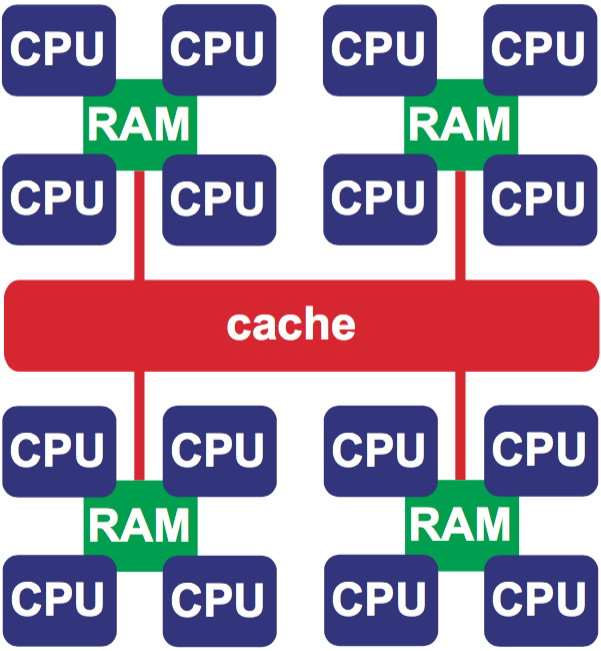
\includegraphics[width=0.6\textwidth]{img/tobias/ccnuma.png}
    	\caption{Arquitetura Paralela ccNUMA heterogênea.}
    	\label{fig:ccnuma}
    \end{figure}
\end{frame}



%\begin{frame}
%    \begin{multicols}{2}
%	
%	    \begin{figure}[h]
%	    	\centering
%	    	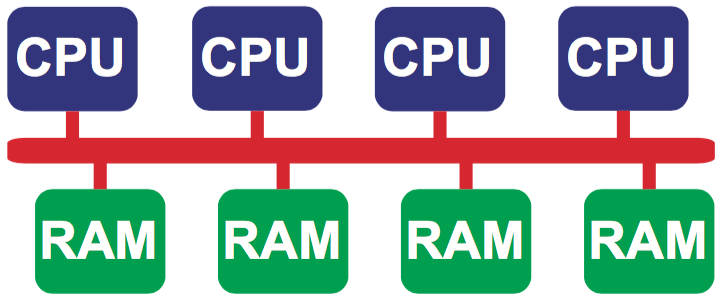
\includegraphics[width=0.42\textwidth]{img/tobias/sm-mimd2.png}
%	    	\caption{Compartilhamento de memória por meio de {\bf 1 único barramento}.}
%	    	\label{fig:sm-mimd2}
%	    \end{figure}
%
%	    \begin{figure}[h]
%	    	\centering
%	    	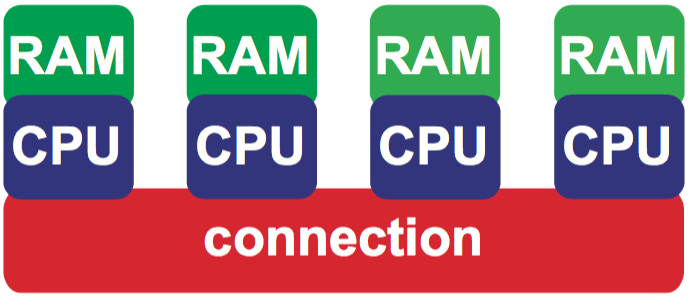
\includegraphics[width=0.42\textwidth]{img/tobias/dm-mimd.png}
%	    	\caption{Distribuição de memória.}
%	    	\label{fig:dm-mimd}
%	    \end{figure}
%
%	\columnbreak
%
%	    \begin{figure}[h]
%	    	\centering
%	    	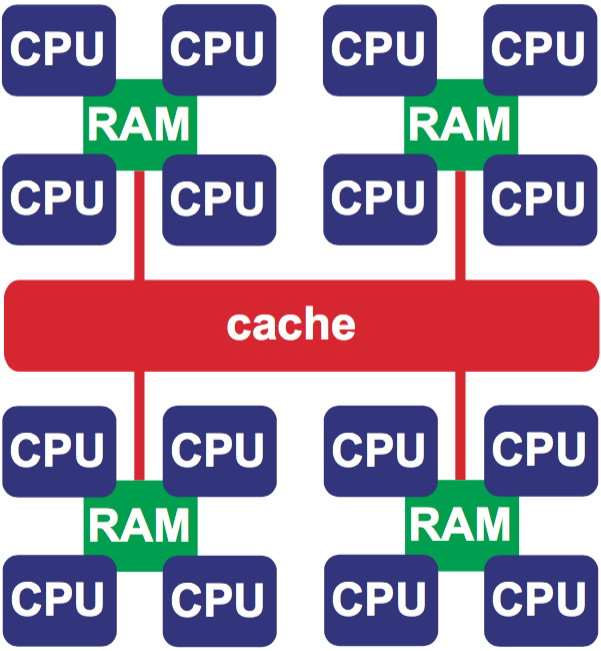
\includegraphics[width=0.42\textwidth]{img/tobias/ccnuma.png}
%	    	\caption{Arquitetura Paralela ccNUMA.}
%	    	\label{fig:ccnuma}
%	    \end{figure}
%
%    \end{multicols}
%
%\end{frame}


%\begin{frame}{ccNUMA}
%    \begin{itemize}
%		\item São conectados entre si criando uma rede de comunicação rápida utilizando um {\bf comutador}.
		
%		    \bigskip
		    
%		\item É fácil utilizar tal como o Memória Compartilhada: 
%		\begin{itemize}
%		    \item Com a vantagem de ser facilmente expansível.
%		\end{itemize}

%		\item Para garantir o desempenho ideal
%		\begin{itemize} 
%			\item Priorizar o uso da {\bf memória local} e não a dos outros módulos.
%		\end{itemize}
%		\item {\bf Módulos} podem ser {\it acoplados/conectados} para obter um sistema maior.	
%	\end{itemize}

%\end{frame}







\begin{frame}{Cluster}
	\begin{itemize}
		\item Clusters são uma forma \textbf{popular} de computação de alta performance.
		\item Consistem em \textbf{vários computadores baratos} conectados entre si.
		\item Conhecidos como \textbf{Rede de \textit{Workstations}} (NOW) e como produto final um Sistema Híbrido
		\begin{itemize}
			\item Os \textbf{nós} teriam \textbf{sistemas de memória compartilhada} formados por \textbf{sistema de memória distribuída}.
		\end{itemize}
	
	\end{itemize}

\end{frame}


\begin{frame}{Cluster}
    \begin{figure}[h]
    	\centering
    	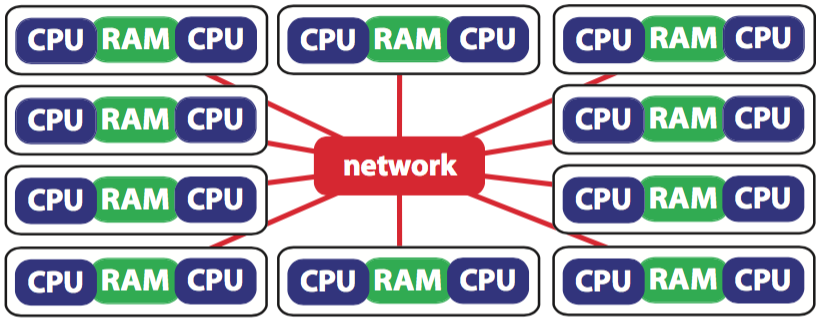
\includegraphics[width=1\textwidth]{img/tobias/cluster.png}
    	\caption{Arquitetura Paralela Cluster.}
    	\label{fig:ccnuma}
    \end{figure}

\end{frame}


\begin{frame}{Cluster}
    \begin{itemize}
%		\item Essa rede distribuída é feita por {\bf redes alta vazão} podendo utilizar comunicações \textbf{Myrinet} ou \textbf{Infiniband}.
%		\begin{itemize}
%			\item \textbf{Gigabit Ethernet} tem alta vazão mas com \textbf{alta latência} no envio dos pacotes.
%			\item Enquanto Gigabit Ethernet possui cerca de $100\mu s$ em latência, Myrinet possui $10 - 20 \mu s$.
%		\end{itemize}
%
%		\item Não é fácil utilizar todo seu poder de processamento:
%		\begin{itemize}
%			\item A comunicação entre nós é lenta pois a comunicação distribuída é naturalmente lenta.
%			%\item Os nós geralmente possui limites de memória\footnote{Arquitetura 32-bit só endereça 4GB e x86-64 possuem 
%			%limitados slots de memória, entre outros possíveis problemas.}.
%		\end{itemize}
%
%%	\end{itemize}
%%
%%\end{frame}
%%
%%
%%\begin{frame}{Cluster}
%%    \begin{itemize}
		\item \textbf{Vantagens:}
		\begin{itemize}
			\item Bem-suscetível para problemas de \textbf{alto nível de paralelismo};
			\item Sua modularidade permite \textbf{modificações} de forma facilitada. 
		\end{itemize}

			\bigskip

		\item Outro tipo de arquitetura é nomeada \textbf{Grid}.
		\begin{itemize}
			\item São sistemas no qual pode utilizar computadores com arquiteturas \textbf{totalmente diferentes};
			\item São espalhados pelo mundo e conectados entre si;
			%\item Podem utilizar a internet como meio de comunicação;
			\item Possuem um alto grau de processamento computacional.
		\end{itemize}

	\end{itemize}

\end{frame}








%\frame{
%    \Huge \color{blue} \bf  \centering Multiple Instruction - Single Data (MISD)
%}
%
%\begin{frame}{Multiple Instruction - Single Data (MISD)}
%	\begin{itemize}
%		\item Não pode ser feita nem pratica ou teoricamente de forma \textbf{sensata}.
%		
%				\bigskip
%		
%		\begin{block}{Openshaw (1999)}
%		    {\it ``Descobrimos que é difícil calcular o porquê você iria fazer `isso', a menos que você seja um cientista da 
%		    computação interessado em computação estranha. É um sistema altamente especializado e restrito e até muitas vezes 
%		    impraticável, pra não dizer inútil como base para uma máquina de uso geral''.}
%		\end{block}
%		
%	\end{itemize}
%
%\end{frame}





\subsection{Multicomputadores e Multiprocessadores}
\begin{frame}{Multicomputadores e Multiprocessadores}
	\begin{multicols}{2}
	
		{\bf Multiprocessador:}
		\begin{itemize}
			\item Existe somente uma memória compartilhada onde é acessada por meio de comandos de (Load e Store).
			\item Não podem ser ampliados facilmente.
			\item UMA e NUMA.
		\end{itemize}
	\columnbreak
		{\bf Multicomputador:}
		\begin{itemize}
			\item Cada processador tem sua memória privada (Memória distribuída).
			\item Utilizam Send e Receive (não Load e Store).
			\item Exemplo:
			\begin{itemize}
				\item Computadores Maciçamente Paralelos\footnote{DM-MIMD não-comuns.};
				\item Clusters\footnote{Centrados e Descentralizados.}.
			\end{itemize}
		\end{itemize}
	            
	\end{multicols}
\end{frame}
\definecolor{bostonuniversityred}{rgb}{0.8, 0.0, 0.0}
\definecolor{seagreen}{rgb}{0.18, 0.55, 0.34}

\section{Redes de Interconexão}

\subsection{Introdução}

\begin{frame}{Redes de Interconexão}
    \begin{itemize}
        \item Um sistema paralelo deve prover um meio de comunicação entre seus processadores, essas são chamadas de \textbf{redes de interconexão}
        \bigskip
        \item Podem ser implementadas de duas maneiras:
        \medskip
        \begin{itemize}
            \item Meio compartilhado;
            \medskip
            \item Meio comutado.
        \end{itemize}
    \end{itemize}
\end{frame}

\subsection{Meio Compartilhado}

\begin{frame}{Meio Compartilhado}
    \begin{columns}
    \column{0.6\linewidth}
        \fontsize{10pt}{7.2}\selectfont
        \begin{itemize}
            \item Um processador envia a mensagem, todos recebem e somente os destinatários interpretam.
            \medskip
            \begin{itemize}
                \item \textbf{Ex}: Ethernet.
            \end{itemize}
            \bigskip
            \item Processadores esperam até que o meio esteja livre para enviar uma mensagem.
            \bigskip
            \item \textbf{Colisão}:
            \medskip
            \begin{itemize}
                \item Ambas mensagens são descartadas;
                \medskip
                \item Após um tempo aleatórios, os remetentes reenviam a mensagem;
                \medskip
                \item \textbf{{\color{bostonuniversityred}Leva a uma perda de performance do meio de comunicação.}}
            \end{itemize}
        \end{itemize}
        \fontsize{10pt}{7.2}\selectfont
        \column[b]{0.4\linewidth}
        \begin{figure}[H]
            \centering
            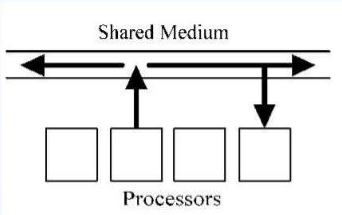
\includegraphics[width=1\linewidth]{img/redes_de_interconexao/shared}
            \caption{Rede compartilhada}
            \label{fig:shared}
        \end{figure}
    \end{columns}
\end{frame}

\subsection{Meio Comutado}

\begin{frame}{Meio Comutado}
    \begin{columns}
        \column{0.6\linewidth}
            \begin{itemize}
                \item Comunicação ponto-a-ponto entre par de processadores.
                \medskip
                \item Cada processador tem seu meio de comunicação individual para o comutador.
                \medskip
                \item {\color{seagreen}\textbf{Vantagens: Comunicação simultânea e escalabilidade.}}
            \end{itemize}
        \column{0.4\linewidth}
            \begin{figure}[H]
                \centering
                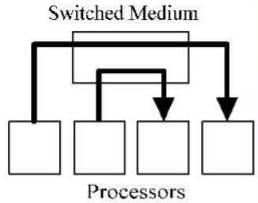
\includegraphics[width=1\linewidth]{img/redes_de_interconexao/switced}
                \caption{Rede comutada}
            \label{fig:sitced}
        \end{figure}
    \end{columns}
\end{frame}

\begin{frame}{Topologia em Redes de Comutação}
    \begin{itemize}
    \only<1>{ \item Topologias são representadas por grafos:
        \begin{itemize}
            \item \textbf{Nós:} Processadores ou comutadores.
            \medskip
            \item \textbf{Arestas:} Meios de comunicação entre os nós.
        \end{itemize}
    \bigskip
}
\only<2>{
    \item Como avaliar a eficiência de uma topologia:
    \medskip
    \begin{itemize}
    \item \textbf{Diâmetro:} Maior distância entre dois nós comutadores. Menor $\rightarrow$ Melhor, provê um limite inferior de complexidade para algoritmos paralelos
    \smallskip
    \item \textbf{Largura de Bisecção:} Número mínimo de arestas que precisam ser removidas para dividir a rede em duas metades. Maior $\rightarrow$ Melhor, provê um limite inferior de complexidade para algoritmos paralelos através da divisão da quantidade de dados que precisam ser transmitidos pela largura de bisecção.
    \smallskip
    \item \textbf{Arestas por nó comutador:} Melhor se a quantidade de arestas por nó comutador é independente do tamanho da rede, provendo escalabilidade.
    \smallskip
    \item \textbf{Comprimento constante de arestas:} Melhor se o comprimento das arestas é independente do tamanho da rede, provendo escalabilidade.
    \end{itemize}
}
    \end{itemize}
\end{frame}

\begin{frame}{Topologias em Redes de Comutação - Exemplos}
	\begin{itemize}
		\item \textbf{Redes 2-D \textit{Mesh}}
		\bigskip
		\begin{itemize}
			\item Grafo direcionado.
			\medskip
			\item Comunicação permitida somente entre vizinhos comutadores.
			\smallskip
			\begin{itemize}
				\item Algumas tem exceções: \textit{wraparound connections.}
			\end{itemize}
		\end{itemize}
	\end{itemize}
	\begin{columns}
		\column{0.75\linewidth}
		\hfill
		\begin{figure}[H]
			\centering
			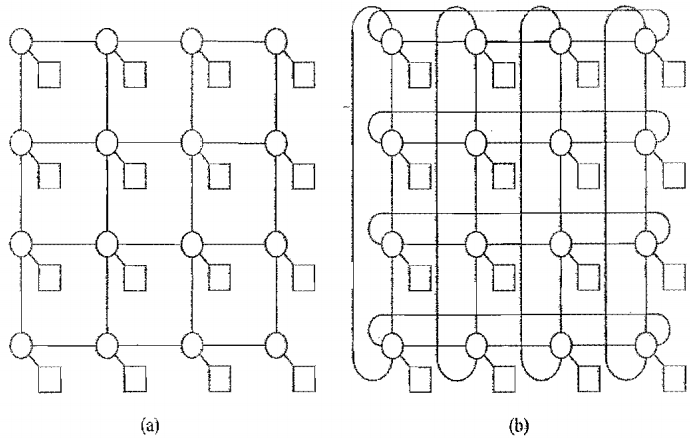
\includegraphics[width=.75\linewidth]{img/redes_de_interconexao/2D-mesh}
			\caption[(a) Rede 2-D mesh simples (b) Rede 2-D mesh com wraparound connections]{(a) Rede 2-D mesh simples (b) Rede 2-D mesh com \textit{wraparound connections}}
			\label{fig:2D-mesh}
		\end{figure}
		\column[b]{0.25\linewidth}
		\begin{itemize}
			\item \textbf{Círculos:} comutadores.
			\smallskip
			\item \textbf{Quadrados:} processadores.
		\end{itemize}
	\end{columns}
\end{frame}

\begin{frame}{Topologias em Redes de Comutação - Exemplos}
	\begin{itemize}
		\item \textbf{Hipercubo}
		\bigskip
		\begin{itemize}
			\item Grafo não direcionado.
			\medskip
			\item Dois nós comutadores são adjacentes se seus \textit{labels} diferem em um \textit{bit}.
		\end{itemize}
	\end{itemize}
	\begin{columns}
		\column{0.75\linewidth}
		\hfill
		\begin{figure}[H]
			\centering
			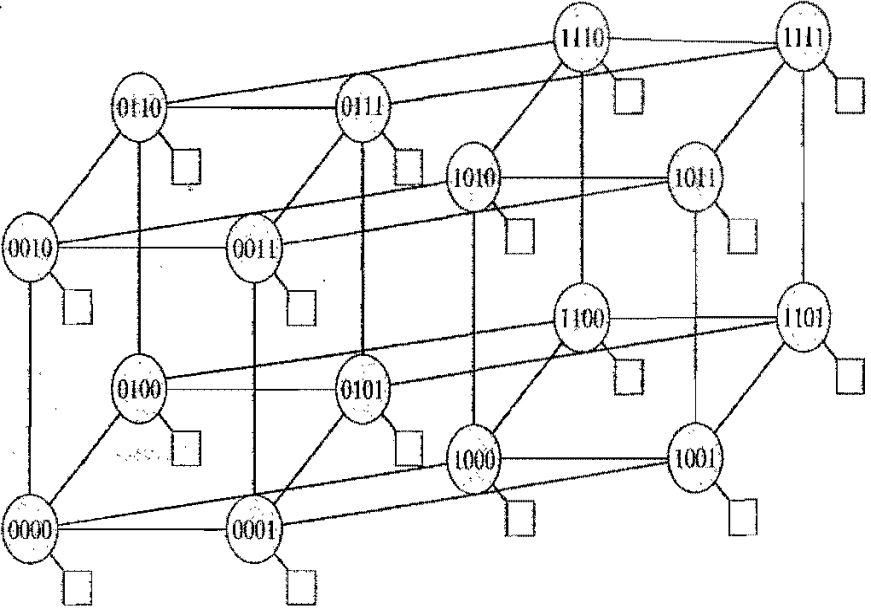
\includegraphics[width=.73\linewidth]{img/redes_de_interconexao/Hyper.png}
			\caption[Hypercubo 4-dimensional]{Hipercubo 4-dimensional}
			\label{fig:hyper}
		\end{figure}
		\column[b]{0.25\linewidth}
		\begin{itemize}
			\item \textbf{Círculos:} comutadores.
			\smallskip
			\item \textbf{Quadrados:} processadores.
		\end{itemize}
	\end{columns}
\end{frame}

\begin{frame}
\begin{center}
\begin{figure}[H]
\centering
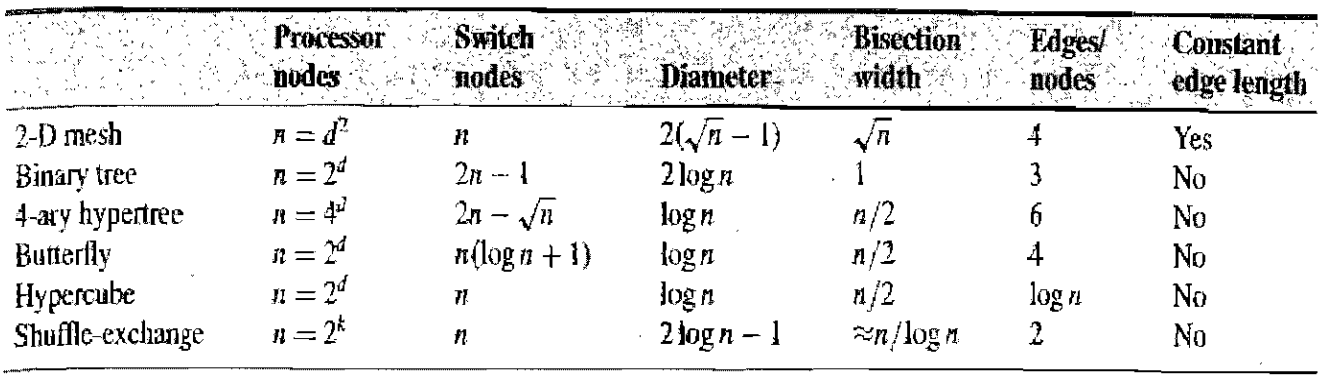
\includegraphics[width=1\linewidth]{img/redes_de_interconexao/compara}
\caption[Comparação entre diferentes topologias]{Comparação entre diferentes topologias}
\label{fig:compara}
\end{figure}
\end{center}

\end{frame}


\section{OpenMP}

\definecolor{bostonuniversityred}{rgb}{0.8, 0.0, 0.0}
\subsection{Introdução}

\begin{frame}{OpenMP (\textit{Open Multi-Processing}) - Introdução}
	\begin{itemize}
		\item Biblioteca que fornece uma API (\textit{Application Programming Interface}) para programação paralela via memória compartilhada.
		\medskip
		\pause
		\item Já existem bibliotecas com a mesma função, como a Pthread \\(\textit{POSIX Threads Programming})\footnote{\url{http://is.gd/FJQyEr}}, por que usar a OpenMP?
		\pause
		\begin{figure}
			\centering
			 \begin{adjustwidth}{-1cm}{}
			\resizebox{\columnwidth}{!}{%
		\begin{tabular}{|c|c|c|}
			\hline
			\cellcolor{gray}{\color{white}\textbf{Requisitos}} & 
			\cellcolor{gray}{\color{white}\textbf{Pthread}} & 
			\cellcolor{gray}{\color{white}\textbf{OpenMP}}\\ \hline
			\textbf{Comportamento de cada thread\footnote{Linha de execução de uma tarefa}} &
			Programador deve especificar manualmente &
			\pbox{3cm}{\vspace{0.1 in}Compilador e sistema de\\ execução lidam\vspace{0.1 in}} \\ \hline
			\textbf{Portabilidade} & \pbox{20cm}{\vspace{0.1 in} Pode ser carregada em qualquer programa,\\ em qualquer compilador,\\ em C/C++\vspace{0.1 in}} & \pbox{20cm}{\vspace{0.1 in}Depende do suporte do\\ compilador.\\OpenMP faz a especificação e os\\ desenvolvedores dos compiladores\\ implementam\vspace{0.1 in}}\\ \hline
			\textbf{Nível de programação} & $\downarrow$ baixo nível & $\uparrow$ alto nível \\ \hline
		\end{tabular}
	}
	\caption {Pthread $\times$ OpenMP}
	 \end{adjustwidth}
		
	\end{figure}
	\end{itemize}
\end{frame}

\begin{frame}{OpenMP - Introdução}
	\begin{itemize}
		\item \textbf{Uso de funções, variáveis globais e macros\footnote{https://gcc.gnu.org/onlinedocs/cpp/Macros.html}:} Inserção do\\ cabeçalho \texttt{omp.h}.
		\pause
		\medskip
		\item Provê uma API baseada em diretivas, chamadas \texttt{pragmas}.
		\medskip
		\begin{itemize}
			\item São instruções especiais do pré-processador de C/C++
			\smallskip
			\item Permitem especificar comportamento não presente por padrão na linguagem.
			\smallskip
			\item \textbf{Portabilidade:} Se o compilador não suporta, a diretiva é ignorada.
			\smallskip
			\item São especificadas em uma linha, caso excedam adiciona-se o caractere de escape \texttt{\textbackslash} ao final da linha.
			\smallskip
			\item \textbf{Forma:} \texttt{\#pragma omp} $<$diretivas$>$.
		\end{itemize}
	\end{itemize}
\end{frame}

\begin{frame}[fragile]
%	\begin{adjustwidth}{0.2cm}{}
	\fontsize{8.5pt}{7.2}\selectfont
\begin{lstlisting}[caption=omp\_hello.c]
#include <stdio.h>
#include <stdlib.h>
#include <omp.h>
void Hello(void);

int main(int argc, char* argv[]) {
	int thread_count = strtol(argv[1], NULL, 10);

	#pragma omp parallel num_threads(thread_count)
	Hello();

	return 0;
}

void Hello(void) {
	int my_rank = omp_get_thread_num();
	int thread_count = omp_get_num_threads();

	printf("Hello from thread %d of %d\n", 
	            my_rank, thread_count);
}
	\end{lstlisting}
	\fontsize{10pt}{7.2}\selectfont	
%\end{adjustwidth}
\end{frame}

\subsection{Compilando e executando}

\begin{frame}[fragile]{OpenMP - Compilando e executando}
	\begin{itemize}
		\item Para compilar com suporte à OpenMP utilizando o \texttt{gcc}\footnote{A OpenMP é suportada no \texttt{gcc} desde a versão 4.2 $<$\url{http://is.gd/MKkNVK}$>$}, adiciona-se o parâmetro \texttt{-fopenmp}:
	\end{itemize}
	\begin{adjustwidth}{-1.6cm}{}
	\fontsize{9pt}{7.2}\selectfont
	\begin{lstlisting}[language=bash]
				$ gcc -g -Wall -fopenmp -o omp_hello omp_hello.c
	\end{lstlisting}
	\fontsize{10pt}{7.2}\selectfont
	\end{adjustwidth}
	\pause
	\begin{itemize}
		\item Executando o programa, especificando 4 \textit{threads} para execução:
	\end{itemize}
	\begin{adjustwidth}{-1.6cm}{}
	\fontsize{9pt}{7.2}\selectfont
	\begin{lstlisting}[language=bash]
				$ ./opm_hello 4
	\end{lstlisting}
	\fontsize{10pt}{7.2}\selectfont
	\end{adjustwidth}
	\pause
	\begin{itemize}
		\item Gerando uma \textbf{possível} saída:
		\medskip
		\begin{itemize}
			\item \textit{Threads} competem por acesso á saída padrão (\texttt{stdout}).
		\end{itemize}
	\end{itemize}
		\begin{adjustwidth}{-1.6cm}{}
			\fontsize{9pt}{7.2}\selectfont
			\begin{lstlisting}[language=bash]
					Hello from thread 1 of 4
					Hello from thread 2 of 4
					Hello from thread 0 of 4
					Hello from thread 3 of 4
			\end{lstlisting}
			\fontsize{10pt}{7.2}\selectfont
		\end{adjustwidth}
\end{frame}

\subsection{Checagem de Erros}

\begin{frame}[fragile]{OpenMP - Checagem de Erros}
	\begin{itemize}
		\item A diretiva \texttt{\# pragma} é ignorada por compiladores que não a suportam, porém caso o compilador não suporte a OpenMP, a diretiva \texttt{\#include <omp.h>} e chamadas de métodos como\\ \texttt{omp\_get\_thread\_num} e \texttt{omp\_get\_num\_threads} vão gerar erros.
		\pause
		\medskip
		\item É importante verificar se o compilador suporta a OpenMP, verifica-se se a macro \texttt{\_OPENMP} está definida:
		\fontsize{8pt}{7.2}\selectfont
\begin{lstlisting}
#ifdef _OPENMP
    #include <omp.h>
#endif
...
#ifdef _OPENMP
    int my_rank = omp_get_thread_num();
    int thread_count = omp_get_num_threads();
#else
    int my_rank = 0;
    int thread_count = 1;
#endif
\end{lstlisting}
\fontsize{10pt}{7.2}\selectfont
	\end{itemize}
\end{frame}

\subsection{Diretivas}

\begin{frame}{OpenMP - Diretivas}
	\begin{itemize}
		\item \texttt{\# pragma omp parallel}:
		\medskip
		\begin{itemize}
			\item Especifica que um número determinado de \textit{threads} devem executar o \textbf{bloco estruturado de código} consecutivo.
			\medskip
			\item \textbf{Bloco estruturado de código:}
			\begin{itemize}
				\item Conjunto de código com um ponto de entrada e um ponto de saída.
				\smallskip
				\item Permite invocação do comando \textbf{exit} no meio do bloco.
				\smallskip
				\item Proíbe qualquer desvio externo que entre no meio do bloco ou que saia para fora do bloco.
			\end{itemize}
			\medskip
			\begin{columns}
				\column{0.55\linewidth}
					\item Cada \textit{thread}:
					\smallskip
					\begin{itemize}
						\item É um \texttt{fork} do programa principal, compartilhando da maioria de seus recursos.
						\smallskip
						\item Possui sus própria pilha de memória e contador de programa.
						\smallskip
						\item Quando completa o trabalho, executa o \texttt{join} e se junta ao processo principal.
					\end{itemize}
					\medskip
					\item Todo esse gerenciamento de \textit{threads} é feito pela OpenMP.
				\column{0.45\linewidth}
					\begin{figure}[H]
						\centering
						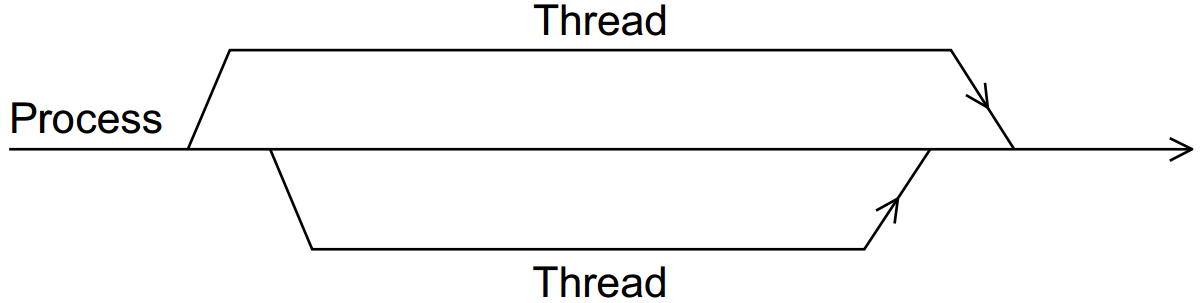
\includegraphics[width=1\linewidth]{img/OpenMP/thread}
						\caption[Fork e Join de duas threads]{\texttt{Fork} e \texttt{Join} de duas \textit{threads}}
						\label{fig:thread}
					\end{figure}
			\end{columns}
		\end{itemize}
	\end{itemize}
\end{frame}

\begin{frame}{OpenMP - Diretivas}
	\begin{itemize}
		\item \texttt{\# pragma omp parallel}:
		\medskip
		\begin{itemize}
			\item Pode ser ou não especificada a quantidade de \textit{threads} a serem executadas.
			\smallskip
			\begin{itemize}
				\item Caso não seja, é determinado em tempo de execução (uma \textit{thread} por \textit{core} disponível.)
				\smallskip
				\item Para especificar uma quantidade $n$ de \textit{threads}, usa-se: \\ \texttt{\# pragma omp parallel num\_threads(n)}
				\smallskip
				\item Alguns sistemas \textbf{podem} limitar a quantidade de \textit{threads} que podem ser executadas.
			\end{itemize}
			\medskip
			\pause
			\item Quando o compilador reconhece a diretiva \texttt{parallel}:
			\begin{itemize}
				\item A \textit{thread} do programa principal continua executando (\textbf{mestre}) e são criadas $n-1$ \textit{threads} (\textbf{escravos}) para executar o bloco de código consecutivo, formando o conjunto de $n$ \textit{threads} chamado \textbf{time}.
				\smallskip
				\item \textbf{Barreira implícita:} Se uma \textit{thread} do \textbf{time} termina a execução do bloco, espera por todas as outras \textit{threads}. Quando todas terminam, as \textit{threads} do tipo \textbf{escravo} são terminadas e o \textbf{mestre} continua executando.
			\end{itemize}
		\end{itemize}
	\end{itemize}
\end{frame}

\subsubsection{Escopo de variáveis}

\begin{frame}{Escopo de variáveis}
	\begin{itemize}
		\item Relembrando, em C/C++:
		\smallskip
		\begin{itemize}
			\item Variáveis declaradas dentro de funções, podem ser usadas apenas dentro das funções (\textbf{escopo local}).
			\smallskip
			\item Variáveis declaradas fora de qualquer função, podem ser usadas em qualquer lugar no arquivo onde foram declaradas (\textbf{escopo global}).
		\end{itemize}
		\medskip
		\pause
		\item Na especificação da OpenMP, variáveis dentro de um bloco executado pela diretiva \texttt{parallel} (pode ser acessada por todas as \textit{threads} do \textbf{time}) tem dois escopos:
		\smallskip
		\begin{enumerate}
			\item \textbf{Compartilhado:} Variáveis declaradas antes fora do bloco estruturado de código que está sendo executado em paralelo, mas que são acessíveis.
			\smallskip
			\item \textbf{Privado:} Variáveis declaradas dentro do bloco estruturado de código que está sendo executado em paralelo. Cada \textit{thread} vai ter sua própria variável declarada em sua pilha de memória.
		\end{enumerate}
	\end{itemize}
\end{frame}

\begin{frame}[fragile]{OpenMP - Diretivas}
	\begin{itemize}
		\item \texttt{\# pragma omp critical}:
		\medskip
		\item Quando múltiplas \textit{threads} tentam acessar o mesmo recurso, acontece o que é chamado de \textbf{condição de corrida}:
		\smallskip
		\begin{itemize}
			\item Se algum dos acessos for para escrita, pode resultar em inconsistência dos dados.
			\smallskip
			\item \textit{Threads} podem ler valor inválidos.
		\end{itemize}
		\medskip
		\pause
		\item O bloco de código contendo o recurso compartilhado é chamado de \textbf{sessão crítica}.
		\medskip
		\pause
		\item Quando uma \textit{thread} está dentro de uma sessão crítica, somente ela pode alterar o recurso (\textbf{exclusão mútua}).
		\medskip
		\pause
		\item Para garantir exclusão mútua à um bloco estruturado de código utilizando a OpenMP, adiciona-se a diretiva \texttt{\#pragma omp critical}
\fontsize{8pt}{7.2}\selectfont
\begin{lstlisting}
...
# pragma omp critical
altera_recurso_compartilhado(recurso);
...
\end{lstlisting}
\fontsize{10pt}{7.2}\selectfont
	\end{itemize}
\end{frame}
\definecolor{bostonuniversityred}{rgb}{0.8, 0.0, 0.0}
\subsection{Cláusula de Redução}

\begin{frame}[fragile]{OpenMP - Cláusula de Redução}
	\begin{itemize}
		\item Suponhamos que temos a seguinte variável:
	\end{itemize}
\begin{lstlisting}
...
double resultado_global = 0.0;
...
\end{lstlisting}
\pause
	\begin{itemize}
		\item Agora, suponhamos que temos a seguinte função, que calcula algum resultado que será armazenado em (\texttt{resultado\_global}) e desejamos paralelizá-la com a diretiva \texttt{parallel}:
	\end{itemize}
\begin{lstlisting}
...
calcula_resultado();
...
\end{lstlisting}
\end{frame}

\begin{frame}[fragile]
	\begin{itemize}
		\item Essa função pode ser implementada de duas maneiras distintas:
	\end{itemize}
\fontsize{7.5pt}{7.2}\selectfont
\begin{lstlisting}[caption=Implementação 1]
double resultado_global = 0.0;
...
void calcula_resultado(double *resultado_global);
...
# pragma omp parallel num_threads(thread_count)
calcula_resultado(&resultado_global)
\end{lstlisting}
\pause
\begin{lstlisting}[caption=Implementação 2, label=impl2]
double resultado_global = 0.0;
double calcula_resultado();
# pragma omp parallel num_threads(thread_count)
{
	# pragma omp critical
	resultado_global += calcula_resultado();
}
\end{lstlisting}
\pause
\fontsize{10pt}{7.2}\selectfont
\begin{itemize}
	\item \textbf{{\color{bostonuniversityred} Alguém vê algum problema com a implementação 2?}}
\end{itemize}

\end{frame}

\begin{frame}[fragile]{OpenMP - Cláusula de Redução}
\begin{itemize}
	\item Devido à sessão crítica, cada chamada de \texttt{calcula\_resultado} pode ser invocada somente por uma \textit{thread} por vez, ou seja, \textbf{sequencialmente}.
	\medskip
	\pause
	\item Uma possível solução:
\end{itemize}
\fontsize{8pt}{7.2}\selectfont
\begin{lstlisting}
...
double resultado_global = 0.0;
...
double calcula_resultado();
...
# pragma omp parallel num_threads(thread_count)
{
	double resultado_privado = 0.0;
	resultado_privado += calcula_resultado();
	# pragma omp critical
	resultado_global += resultado_privado;
}
\end{lstlisting}
\fontsize{10pt}{7.2}\selectfont
\end{frame}

\begin{frame}[fragile]{OpenMP - Cláusula de Redução}
\begin{itemize}
	\item Essa é uma possível solução, mas a OpenMP provê uma solução mais limpa e elegante através da especificação de uma \textbf{variável de redução}.
	\smallskip
	\begin{itemize}
		\item Variável que interage com um \textbf{operador de redução}.
		\smallskip
		\begin{itemize}
			\item Operador binário (\textbf{Ex:} Adição e Multiplicação).
			\smallskip
			\item \textbf{Redução:} Cômputo que aplica o mesmo operador de redução à uma sequência de operandos para conseguir um único resultado.
		\end{itemize}
	\end{itemize}
	\medskip
	\pause
	\item Para tal, adiciona-se a cláusula \texttt{reduction} à diretiva \texttt{parallel}:
\end{itemize}
\fontsize{8pt}{7.2}\selectfont
\begin{lstlisting}
...
double resultado_global = 0.0;
...
double calcula_resultado();
...
# pragma omp parallel num_threads(thread_count) \
reduction(+: resultado_global)
{
	resultado_global += calcula_resultado();
}
\end{lstlisting}
\fontsize{10pt}{7.2}\selectfont
\end{frame}

\begin{frame}{OpenMP - Cláusula de Redução}
\begin{itemize}
	\item Internamente, o compilador vai criar uma variável privada para cada \textit{thread} dentro de uma seção crítica.
	\medskip
	\pause
	\item Nesse exemplo, todas as variáveis privadas são inicializadas em \texttt{0.0}.
	\medskip
	\pause
	\item Sintaxe da cláusula de redução:\\ \texttt{reduction(<operador>: <lista de variáveis>) }.
	\smallskip
	\begin{itemize}
		\item Operadores válidos:$ +, *, -, \&, |, $\textasciicircum$, \&\&, ||$.
	\end{itemize}
\end{itemize}
\end{frame}

\begin{frame}[fragile]{OpenMP - Cláusula de Redução}
\begin{itemize}
	\item Alguns problemas com a cláusula de redução:
	\medskip
	\begin{itemize}
		\item Operação de subtração não é associativa\footnote{Diferente comportamento em uma expressão com e sem parênteses.} ou comutativa, por exemplo:
	\end{itemize}
\fontsize{8pt}{7.2}\selectfont
\begin{lstlisting}
resultado = 0;
for (i = 1; i <= 4; i++)
	resultado -= i;
\end{lstlisting}
\fontsize{10pt}{7.2}\selectfont
	\begin{itemize}
		\item A versão sequencial desse código retorna $-10$.
		\medskip
		\item Separando as operações em duas \textit{threads}, onde a \textit{thread} 0 executa $(-1) + (-2)  =-3$ e a \textit{thread} 1 executa $(-3) + (-4)=-7$.
		\medskip
		\item O resultado final será $-3-(-7) =$ {\color{bostonuniversityred}$4$}.
		\medskip
		\item O correto seria: $-3+(-7) = -10$
	\end{itemize}	
\bigskip
\pause
\item A aritmética de ponto flutuante também não é associativa:\\ $((a + b) + c)$ e $(a +(b + c))$ podem não ter o mesmo resultado exato.
\end{itemize}
\end{frame}

%\section{Cláusula de Redução}

\frame{
    \Huge \color{blue} \bf  \centering Reduction
}

\begin{frame}[fragile]{Reduction - Introdução}
	\begin{lstlisting}
void Trap(double a, double b, int n, double* global_result_p);
	\end{lstlisting}

	\begin{itemize}
		\item Esta, provavelmente, não seria a chamada de função que utilizaríamos.

				\pause

		\item Utilizaríamos algo como:
	\end{itemize}

	\begin{lstlisting}
double Trap(double a, double b, int n);
	\end{lstlisting}

			\pause

	\begin{itemize}
		\item Assim, teríamos a função:
	\end{itemize}

	\begin{lstlisting}
global_result = 0.0;
# pragma omp parallel num_threads(thread_count) 
{
    #   pragma omp critical
    global_result += Trap(double a, double b, int n); 
}
	\end{lstlisting}

			\pause

	\begin{itemize}
		\item Mas há algo errado nesta função. O quê?
	\end{itemize}
\end{frame}




\begin{frame}[fragile]{Reduction - Introdução}
	\begin{lstlisting}
global_result = 0.0;
# pragma omp parallel num_threads(thread_count)
{
	double my_result = 0.0;
	my_result += Trap(double a, double b, int n); 
	#	pragma omp critical
	global_result += my_result;
}
	\end{lstlisting}

	\begin{enumerate}
		\item A {\bf chamada} está {\bf fora da seção crítica}.
		\item As threads poderão ser chamadas/executadas simultaneamente.
	\end{enumerate}
\end{frame}




\begin{frame}[fragile]{Reduction - Conceitos}
	\begin{itemize}
		\item OpenMP provê outras alternativas para esse tipo de situação.
		\item É denominado {\bf \textit{redução} da variável}.
		\begin{itemize}
			\item {\bf Reduction Operator:} Qualquer tipo de operador bináio em C/C++ (\verb!+, *, -, &, | , ^, &&, ||!);
			\item {\bf Reduction:} Computação que aplica repetidadamente o mesmo operador para uma sequência de operandos para pegar um simples resultado;
			\item {\bf Reduction Variable:} Variável de armazemamento (\verb&global_result&).
		\end{itemize}
	\end{itemize}

	\begin{lstlisting}
int sum = 0;
for (i = 0; i < n; i++)
	sum += A[i];
	\end{lstlisting}

	\begin{itemize}
		\item Em OpenMP, é possível realizar uma \textbf{redução} de uma específica variável ({\bf variável redutiva}) que utiliza um operador binário (\textbf{operador redutível}) por meio de diretivas.
	\end{itemize}
\end{frame}




\begin{frame}[fragile]{Reduction - Aplicação}
	\begin{lstlisting}
global_result = 0.0;
# pragma omp parallel num_threads(thread_count)
{
	double my_result = 0.0;
	my_result += Trap(double a, double b, int n); 
	#	pragma omp critical
	global_result += my_result;
}
	\end{lstlisting}

	\begin{itemize}
		\item Poderia ser reescrito como:
	\end{itemize}

	\begin{lstlisting}
global_result = 0;
# pragma omp parallel num_threads(thread_count) \
		reduction(+: global_result)
global_result += Trap(double a, double b, int n);
	\end{lstlisting}
\end{frame}




\begin{frame}[fragile]{Reduction - Aplicação}
	\begin{lstlisting}
global_result = 0;
# pragma omp parallel num_threads(thread_count) \
		reduction(+: global_result)
global_result += Trap(double a, double b, int n);
	\end{lstlisting}

			\bigskip

	\begin{enumerate}
		\item Cria-se uma variável privada para cada thread de uma team;
		\item Os dados de cada thread são gravados nestas;
		\item Também cria-se uma seção crítica para adição dessas com o valor final.
	\end{enumerate}

			\pause

	\begin{itemize}
		\item A Redução de uma variável \verb%float% ou \verb%double% pode resultar em valores ligeiramente diferentes.
		\begin{itemize}
			\item $a + (b + c)$ pode não ter o mesmo valor que usar $(a + b) + c$.
		\end{itemize}
		\item Quando uma variável é reduzida, automaticamente é compartilhada.
	\end{itemize}
\end{frame}




\begin{frame}[fragile]{Reduction - Aplicação}

	\begin{lstlisting}
global_result = 0;
# pragma omp parallel num_threads(thread_count) \
		reduction(+: global_result)
global_result += Trap(double a, double b, int n);
	\end{lstlisting}

	\begin{itemize}
		\item possui a mesma função que:
	\end{itemize}

	\begin{lstlisting}
global_result = 0.0;
# pragma omp parallel num_threads(thread_count)
{
	double my_result = 0.0;
	my_result += Trap(double a, double b, int n); 
	#	pragma omp critical
	global_result += my_result;
}
	\end{lstlisting}

	\begin{itemize}
		\item As variáveis privadas são inicializadas de acordo com o operando
				\pause
		\begin{itemize}
			\item Operando redutor \verb&+& inicializa as variáveis com o valor 0;
			\item Operando redutor \verb&*& inicializa as variáveis com o valor 1.
		\end{itemize}
	\end{itemize}
\end{frame}

\subsection{Diretiva {\tt parallel for}}

\begin{frame}[fragile]{Diretiva {\tt parallel for}}
	\begin{itemize}
		\item Também existe uma diretiva que torna possível paralelizar {\bf estruturas de repetição}.
				\pause
		\item Temos o seguinte bloco a ser executado:
	\end{itemize}

%	\begin{lstlisting}
%h = (b - a) / n;
%approx = (f(a) + f(b)) / 2.0;
%for (i = 1; i <= n - 1; i++)
%	approx += f(a + i * h); 
%approx = h * approx;
%	\end{lstlisting}


\begin{lstlisting}
somatorio = 0;
for (i = 0; i < n; i++)
	somatorio += calcula(a + i * h); 
somatorio = h * somatorio;
\end{lstlisting}

		\pause

	\begin{itemize}
		\item Com a diretiva para paralelização de \textit{loop}:
	\end{itemize}

%	\begin{lstlisting}
%h = (b - a) / n;
%approx = (f(a) + f(b)) / 2.0;
%# pragma omp parallel for num_Threads(thread_count) \
%	reduction(+: approx) 
%for (i = 1; i <= n - 1; i++)
%	approx += f(a + i * h);
%approx = h * approx;
%	\end{lstlisting}

\begin{lstlisting}
somatorio = 0;
# pragma omp parallel for num_Threads(thread_count) \
	reduction(+: somatorio) 
for (i = 0; i < n; i++)
	somatorio += calcula(a + i * h); 
somatorio = h * somatorio;
\end{lstlisting}

\end{frame}




\begin{frame}{Diretiva {\tt parallel for}}
	\begin{itemize}
	    \setlength\itemsep{1em}
		\item Como o {\tt parallel}, o {\tt parallel for} realiza um {\it fork} de um {\bf time} de \textit{Threads} para executar o bloco seguinte.
		\item {\bf Obrigatoriamente}, deve-se utilizar o comando {\tt for} para tal.
		\item O que ocorre internamente é que:
		\begin{itemize}
	        \setlength\itemsep{0.7em}
			\item {\bf O sistema} paraleliza o loop {\bf dividindo em iterações de loop};
			\item Os blocos são {\bf divididos} por \textit{Threads}:
			\begin{itemize}
				\item $i / thread\_count$;
				\item {\bf \textit{Thread} 0} fica com o {\bf bloco 0};
				\item {\bf \textit{Thread} 1} fica com o {\bf bloco 1}...
			\end{itemize}

		\end{itemize}

	\end{itemize}

\end{frame}


\begin{frame}{Diretiva {\tt parallel for}}
	\begin{itemize}
	    \setlength\itemsep{1em}
		\item Diferencia-se dos {\tt parallel} pois:
		\begin{itemize}
	        \setlength\itemsep{0.6em}
			\item Este necessita ser {\bf dividido entre os \textit{Threads} pelo próprios \textit{Threads}} o que não ocore com o {\tt parallel for};
			\begin{itemize}
				\item No {\tt parallel} as \textit{Threads} distribuiem o trabalho entre si;
				\item No {\tt parallel for} o sistema realiza a distribuição delas.
			\end{itemize}
			\item Todas as variáveis do {\tt parallel} são compartilhadas. Já no {\tt parallel for} são todas {\bf particulares}\footnote{\bf Inclusive o {\tt i}.}.
		\end{itemize}

		\item Realizar a {\bf \textit{redução} da variável somadora} protegendo-a com a {\bf seção crítica}
		\begin{itemize}
			\item Se a variável {\tt i} fosse compartilhada, deveria proteger usando seção crítica ao realizar o {\tt i++}.
		\end{itemize}

	\end{itemize}

\end{frame}

\begin{frame}[fragile]{Diretiva {\tt parallel for} - Ressalvas}
	\begin{itemize}
		%\item O uso do {\tt parallel for} possui várias ressalvas.
		\item {\bf Não é possível paralelizar} {\tt while} ou {\tt do-while}

			\pause

		\begin{itemize}
			\item Isto não significa uma limitação;
			\item Qualquer código pode ser convertido em código equivalente que utiliza um loop {\tt for}.
		\end{itemize}

			\bigskip
			\pause

		\item Compilador que suporta OpenMP, paraleliza loops que tenham {\bf limite de iterações}. São eles:
		\begin{itemize}
			\item Definição pelo \verb% for (. . .; . . .; . . .) % ; e
			\item Antes da execução do loop.
		\end{itemize}
	\end{itemize}
\end{frame}




\begin{frame}[fragile]
	\begin{itemize}
		\item Só paraleliza loops na {\bf forma canônica}:
	\end{itemize}
$
\mathtt{for} \left(
		\begin{array}{c}
			\mathtt{index = start}
		\end{array}
		;
		\begin{array}{c}
			\mathtt{index > end} \\
			\mathtt{index >= end} \\
			\mathtt{index <= end} \\
			\mathtt{index < end} \\
		\end{array}
		;
		\begin{array}{c}
			\mathtt{index++} \\
			\mathtt{index--} \\
			\mathtt{--index} \\
			\mathtt{++index} \\
			\mathtt{index += incr} \\
			\mathtt{index -= incr} \\
			\mathtt{index = index + incr} \\
			\mathtt{index = incr + index} \\
			\mathtt{index = index - incr} 
		\end{array}
	\right)
$
			\\[1.2cm]
			\pause

	\begin{itemize}
		\item Exemplos de códigos que {\bf \textit{não} podem ser paralelizados}:
	\end{itemize}

	\begin{multicols}{2}
		Loop Infinito
		\begin{lstlisting}
for ( ; ; ) {

}
		\end{lstlisting}

	\columnbreak
		Loop com interrupção
		\begin{lstlisting}
for (i = 0; i < n; i++) {
	if ( . . . ) break;
}
		\end{lstlisting}	

	\end{multicols}
\end{frame}


\begin{frame}[fragile]{Diretiva {\tt parallel for}  - Dependência de Dados}
	\begin{itemize}
		\item Mas quando o loop falha sobre uma das regras citadas?

			\pause

	\begin{lstlisting}
for (i = 0; i < n; i++)
	if (A[i] == key) return i;
return -1;
	\end{lstlisting}

			\pause

		\item O compilador \verb&gcc& rejeitará o comando de paralelismo retornando erro:

	\end{itemize}

		\bigskip	

	\verb&Line 2: error: invalid exit from OpenMP structured block&
\end{frame}




\begin{frame}[fragile]{Diretiva {\tt parallel for}  - Dependência de Dados}
	\begin{lstlisting}
fibo[0] = fibo[1] = 1;
# pragma omp parallel for num_Threads(thread_count)
for (i = 2; i < n; i++)
	fibo[i] = fibo[i-1] + fibo[i-2];
	\end{lstlisting}

		\pause

	\begin{itemize}
		\item Será criado um executável sem qualquer alerta.

			\pause
%	\end{itemize}
%\end{frame}
%
%
%\begin{frame}[fragile]{Diretiva {\tt parallel for}  - Dependência de Dados}
%	\begin{itemize}
		\item Exemplo utilizando 2 \textit{Threads} para 10 números:
		\begin{enumerate}
			\item \textit{1 1 2 3 5 8 13 21 34 55};
			\begin{itemize}
				\pause
				\item Uma \textit{Thread} ficou com o 2 ao 5 e outra com 6 ao 9;
				\item E a segunda só começou depois que a primeira terminou.
			\end{itemize}

				\pause

			\item \textit{1 1 2 3 5 8 0 0 0 0}.
			\begin{itemize}
				\pause
				\item Uma \textit{Thread} ficou com o 2 ao 5 e outra com 6 ao 9;
				\pause
				\item A segunda terminou primeiro a execução;
				\item {\tt fibo[4] = 0} e  {\tt fibo[5] = 0}.
			\end{itemize}
		\end{enumerate}

            \pause
            \bigskip

		\item Entretanto, os resultados {\bf serão imprevisíveis}.
	\end{itemize}
\end{frame}




\begin{frame}[fragile]{Diretiva {\tt parallel for}  - Dependência de Dados}
	\begin{itemize}
	    \setlength\itemsep{1.1em}
		\item Isso pois o compilador que suporta OpenMP:
		\begin{itemize}
	    \setlength\itemsep{0.8em}
			\item Não verifica dependências durante as interações no loop;
			\item Loops que necessitam de {\bf valor de iterações passadas}, geralmente, {\bf não podem ser paralelizados} pelo compiladores.
		\end{itemize}
		\item A dependência do {\tt fibo[6]} com o {\tt fibo[5]} é chamada de {\bf Dependência de dados}.
		\item Desde que o valor de {\tt fibo[5]} for calculado em uma interação e o resultado usado em outra {\bf subsequente}, então a dependência as vezes é chamado de {\bf \textit{Loop-Carried Dependence}}.
	\end{itemize}
\end{frame}



\begin{frame}[fragile]{Diretiva {\tt parallel for} - Encontrando \textit{Loop-Carried Dependence}}
	\begin{itemize}
		\item Ao utilizar o {\tt parallel for}, deve-se ficar atento somente aos \textit{Loop-Carried Dependence}.
	\end{itemize}

		\bigskip

	\begin{lstlisting}
for (i = 0; i < n; i++) {
	x[i] = a + i*h;
	y[i] = exp(x[i]);
}
	\end{lstlisting}

		\pause

	\begin{itemize}
		\item Esse código possui dependência de dados entre as linhas mas {\bf não é um problema para a paralelização}.
	\end{itemize}

%	\begin{itemize}
%		\item Deve-se preocupar {\it somente} com variáveis que são {\bf lidas ou gravadas em uma iteração} e {\bf escrita em outra}.
%	\end{itemize}
\end{frame}





\section{Exemplo}
\frame{
    \Huge \color{blue} \bf  \centering Estimando $\pi$ Com Paralelismo
}

\begin{frame}[fragile]{Exemplo da estimação de $\pi$}
	\begin{itemize}
		\item Como seria feito uma estimação com codificação paralela utilizando a fórmula: 
		$$\pi = 4\Bigg[ 1 - \frac{1}{3} + \frac{1}{5} - \frac{1}{7} + \dots \Bigg] = 4 \sum\limits_{k=0}^\infty \frac{(-1)^k}{2k+1}.$$
	\end{itemize}

		\pause

	\begin{lstlisting}
double factor = 1.0, sum = 0.0;
# pragma omp parallel for num_Threads(thread_count) \
	reduction(+:sum)
for (k = 0; k < n; k++) {
	sum += factor/(2*k+1);
	factor = -factor;
}
pi_approx = 4.0 * sum;
	\end{lstlisting}

	\begin{itemize}
		\item {\bf Relembrando:} Deve-se preocupar somente com variáveis que são lidas ou gravadas em uma iteração e escrita em outra.
	\end{itemize}
\end{frame}




\begin{frame}[fragile]{Exemplo da estimação de $\pi$}
	\begin{lstlisting}
double factor = 1.0, sum = 0.0;
# pragma omp parallel for num_Threads(thread_count) \
	reduction(+:sum)
for (k = 0; k < n; k++) {
	sum += factor/(2*k+1);
	factor = -factor;
}
pi_approx = 4.0 * sum;
	\end{lstlisting}

	\begin{itemize}
		\item É notável que existe uma dependência na variável {\tt factor}.
				\pause
		\begin{itemize}
		    \item Atualizar o valor na linha 6 na iteração $k$ e incrementar o {\tt sum} na linha 5 interação $k+1$ é um \textit{Loop-Carried Dependence}.
		\end{itemize}
	\end{itemize}
\end{frame}



\begin{frame}[fragile]{Exemplo da estimação de $\pi$}
	\begin{itemize}
		\item Trocaremos:
	\end{itemize}
	\begin{lstlisting}
sum += factor/(2*k+1);
factor = -factor;
	\end{lstlisting}

	\begin{itemize}
		\item por
	\end{itemize}
	\begin{lstlisting}
if (k % 2 == 0)
	factor = 1.0;
else 
	factor = -1.0
sum += factor/(2*k+1);
	\end{lstlisting}
\end{frame}





\begin{frame}[fragile]{Exemplo da estimação de $\pi$}
	\begin{lstlisting}
if (k % 2 == 0)
	factor = 1.0;
else 
	factor = -1.0
sum += factor/(2*k+1);
	\end{lstlisting}

	\begin{itemize}
		\item Elimina-se a dependência de loop.

			\pause

		\item Mas se executar-mos o programa, ainda {\bf continuará} a exibir resultado errôneos:
		\begin{itemize}
			\item Qualquer variável declarada antes do loop, é {\bf compartilhada} entre as \textit{Threads};
			\item E com isso, {\tt fator} é compartilhado. 
			\begin{itemize}
				\item Uma \textit{Thread} pode definir o valor de 1 e outra logo em seguida redefine para -1 sem que tenha utilizado.
			\end{itemize}
			\item Deve garantir que cada segmento tem sua própria cópia do fator;
			\item Adiciona-se uma cláusula {\tt private} à diretiva.
		\end{itemize}
	\end{itemize}
\end{frame}


\begin{frame}[fragile]{Exemplo da estimação de $\pi$}

	\begin{lstlisting}
double factor = 1.0, sum = 0.0;
# pragma omp parallel for num_Threads(thread_count) \
	reduction(+:sum) private(factor)
for (k = 0; k < n; k++) {
	if (k % 2 == 0)
		factor = 1.0;
	else 
		factor = -1.0
	sum += factor/(2*k+1);
}
pi_approx = 4.0 * sum;
	\end{lstlisting}
\end{frame}







\begin{frame}[fragile]{Outras Diretivas para Escopo}
	\begin{itemize}
		\item Ao invés de deixar o compilador dicidir qual o âmbito de cada variável, é uma boa prática decidirmos nós mesmo (programadores).
		\item OpenMP oferece uma cláusula chamada {\tt default} pra que isso seja definido.
		\item Ao utilizar essa diretiva, o compilador exigirá que definemos o escopo de cada variável que usamos no bloco.
			\bigskip
		\item Variáveis que são usadas por todas as \textit{Threads} e que não são modificadas, podem, seguramente, ser definidas como compartilhadas.
	\end{itemize}

\end{frame}





\begin{frame}[fragile]{Outras Diretivas para Escopo}
	\begin{lstlisting}
double factor = 1.0, sum = 0.0;
# pragma omp parallel for num_Threads(thread_count) \
	default(none) reduction(+:sum) private(k, factor) \
	shared(n)

for (k = 0; k < n; k++) {
	if (k % 2 == 0)
		factor = 1.0;
	else 
		factor = -1.0
	sum += factor/(2*k+1);
}
pi_approx = 4.0 * sum;
	\end{lstlisting}
\end{frame}





\frame{\titlepage}
\end{document}